\documentclass[11pt]{article}
\usepackage[letterpaper,margin=1in]{geometry}
\usepackage{amsmath,amssymb}
\usepackage{booktabs}
\usepackage{graphicx}
\usepackage{setspace}
\usepackage[hidelinks]{hyperref}
\usepackage{authblk}
\usepackage{xcolor}
\usepackage{titlesec}
\usepackage[numbers,sort&compress]{natbib}

\titleformat*{\section}{\large\bfseries}
\titleformat*{\subsection}{\normalsize\bfseries}

\title{\textbf{Selection on Testing Engagement: A Structural Bias in\\
Cross-Sectional Incidence Estimation Using Recency Assays}}

\author[1]{A.C. Demidont, DO, AAHIVS}
\affil[1]{Nyx Dynamics LLC, Philadelphia, PA 19107. ORCID: 0000-0002-9216-8569.\\
Correspondence: \texttt{ac.demidont@nyxdynamics.com}}

\date{Manuscript draft --- not for distribution}

\begin{document}
\maketitle
\onehalfspacing

\begin{center}
\fbox{\begin{minipage}{0.92\textwidth}
\small
\textbf{Abstract}

\vspace{0.3em}
\textbf{Background.} Cross-sectional HIV incidence estimation using recent-infection testing algorithms (RITAs) underpins counterfactual-controlled pre-exposure prophylaxis (PrEP) efficacy trials. The Kassanjee estimator assumes closed-system observability: that every recently-infected individual within the recency window is equally present at screening. Populations experiencing structural censoring---competing-risk hazards from overdose, incarceration, displacement, and related mechanisms---violate this assumption in a systematic and directional manner.

\textbf{Methods.} We derive the effective mean duration of recent infection under structural censoring, $\Omega^*(\gamma) = \int_0^T P_R(t)\,S_c(t)\,dt$, and the joint bias factor on the reported incidence rate ratio (IRR) incorporating both screening-cohort and intervention-arm observation probabilities. We identify the standard 90-day no-prior-testing eligibility criterion, common to Phase 3 PrEP trials including PURPOSE 1 (NCT04994509) and PURPOSE 2 (NCT04925752), as a selection mechanism operating on the same axis that drives the competing-risk hazard. We apply the framework to 34 high-burden US metropolitan areas using AIDSVu 2023 surveillance data with late-diagnosis percentage as the empirical proxy for structural hazard.

\textbf{Results.} Across 34 MSAs, the Kassanjee denominator is inflated by 8.7\%--27.3\%, with monotone scaling in late-diagnosis percentage. The joint IRR bias factor $B_{\mathrm{IRR}}$ ranges from 0.97 to 0.999, attenuating reported IRRs by up to 3.1\% in the highest-severity cohort. The direction is consistent across the empirical range: reported IRRs understate true IRRs, making interventions appear artificially superior in populations with elevated structural hazard and correspondingly reduced trial retention.

\textbf{Conclusions.} The Kassanjee/Gao cross-sectional incidence estimator produces systematically biased point estimates when applied to populations with elevated structural censoring, and the bias is structurally guaranteed rather than merely possible when trial-design eligibility criteria select the Incidence Phase cohort on the testing-engagement axis. Correction requires explicit modeling of population-specific hazard using surveillance data; the framework presented here is one such correction, fully reproducible from public data, and generalizes to any RITA-based trial with analogous eligibility structure.
\end{minipage}}
\end{center}

\vspace{1em}

\section{Introduction}

Cross-sectional HIV incidence estimation using recent-infection testing algorithms (RITAs) has become a foundational tool in modern prevention trials, particularly for establishing a counterfactual background incidence rate (bHIV) when randomized placebo control is not ethically feasible. The Kassanjee estimator~\cite{kassanjee2012}, extended with delta-method variance by Gao and colleagues~\cite{gao2021}, has been adopted as the primary analytic framework for counterfactual-controlled pre-exposure prophylaxis (PrEP) efficacy trials, including the pivotal PURPOSE~1 (NCT04994509) and PURPOSE~2 (NCT04925752) trials of long-acting injectable lenacapavir~\cite{bekker2024,kelley2025}.

The estimator's validity rests on a closed-system assumption: that the recency assay's mean duration of recent infection ($\Omega$), calibrated on a validation cohort of documented seroconverters, applies directly to the at-risk population being screened. Specifically, $\Omega$ is defined as
\begin{equation}
\Omega \;=\; \int_0^T P_R(t)\,dt \label{eq:omega_def}
\end{equation}
where $P_R(t)$ is the probability that the assay classifies a specimen as ``recent'' at age-of-infection $t$, and $T$ is the recency cutoff (typically 730 days). This definition implicitly assumes that every individual infected within the window $[0, T]$ is observable at screening---that is, that the probability of being alive, non-incarcerated, housed, and presenting for testing is uniformly 1 across the window.

This assumption is not biologically motivated. It is a convenience of calibration.

In populations experiencing structural censoring---competing-risk hazards from overdose mortality, incarceration, displacement, carceral disruption of healthcare, intimate partner violence, and related mechanisms that disproportionately affect marginalized groups---the closed-system assumption fails in a specific, directional, and quantifiable way. The failure mode is not random noise around a correct central estimate; it is systematic deflation of the estimated background incidence, with deflation magnitude correlated with the very structural vulnerabilities that trial designs ostensibly aim to serve.

This letter formalizes the structural correction and identifies a specific trial-design feature---the standard recency eligibility criterion requiring no prior HIV testing within a specified interval---that structurally guarantees the bias rather than merely permitting it. The 90-day no-testing inclusion criterion common to Phase 3 PrEP trials selects the bHIV cohort specifically on the axis (testing engagement) that drives the competing-risk hazard heterogeneity. The calibration-to-deployment mismatch that results is not an artifact of sampling variability; it is a direct consequence of how the Incidence Phase is constructed.

We derive the effective MDRI under structural censoring, $\Omega^*(\gamma)$; derive the joint bias factor on the reported incidence rate ratio incorporating both screening-cohort and intervention-arm observation probabilities; quantify the amplification introduced by the testing-exclusion selection; and apply the framework to 34 high-burden US metropolitan areas using publicly available AIDSVu 2023 surveillance data~\cite{aidsvu2023}, with late-diagnosis percentage as the empirical proxy for testing-avoidance hazard. The correction can be implemented prospectively in any RITA-based trial SAP without access to proprietary data; the framework applies to any cross-sectional incidence estimator with analogous eligibility structure.

\section{The survival-biased effective MDRI}

\subsection{Effective MDRI under structural censoring}

Let $\gamma(t)$ denote the instantaneous hazard of structural censoring at time $t$ post-infection---the per-unit-time probability of transition into an unobservable state via death, incarceration, long-distance displacement, prolonged hospitalization, or any mechanism that removes the individual from the screening pool. Let $S_c(t) = \exp\!\left(-\int_0^t \gamma(u)\,du\right)$ denote the corresponding survival function.

The \emph{effective} mean duration of recent infection, conditional on the population's structural hazard profile, is
\begin{equation}
\Omega^*(\gamma) \;=\; \int_0^T P_R(t)\,S_c(t)\,dt \label{eq:omega_star}
\end{equation}
This is the joint probability, integrated over the recency window, that an individual infected at time 0 (i) tests recent at age $t$ and (ii) remains observable at screening. Since $S_c(t) \leq 1$ pointwise and strictly less than 1 whenever $\gamma > 0$ on a set of positive measure, $\Omega^*(\gamma) < \Omega$ identically for any population experiencing structural censoring. This is a distribution-free result: it requires no parametric form for $\gamma$ or $P_R$.

Under a piecewise-constant hazard approximation with $\gamma$ constant over the recency window and an exponential approximation $P_R(t) \approx P_0\exp(-t/\tau)$ with $\tau \approx \Omega$ for the Sedia LAg-EIA calibration~\cite{sedialag}, a closed-form correction obtains:
\begin{equation}
\Omega^*(\gamma) \;\approx\; \frac{\Omega}{1 + \gamma\tau} \label{eq:omega_closed}
\end{equation}
For $\gamma$ on the order of $10^{-4}$ per day (general population) through $10^{-3}$ per day (structurally marginalized populations) and $\tau = 173$ days, this yields $\Omega^*/\Omega$ ratios spanning 0.85 to 0.98---a deflation range of 2\% to 15\%.

\subsection{Consequence for the Kassanjee point estimate}

Substituting $\Omega^*(\gamma)$ into the Gao et al.\ 2021 cross-sectional incidence estimator,
\begin{equation}
\hat\lambda_0 \;=\; \frac{N_{\mathrm{rec}} - \beta N_+}{N_-\,(\Omega - \beta T)} \label{eq:kassanjee}
\end{equation}
when the trial applies the nominal validation-cohort $\Omega$ while the enrolled cohort experiences $\gamma > 0$, the expected observed recent-infection count $E[N_{\mathrm{rec}}]$ reflects $\Omega^*(\gamma)$ rather than $\Omega$:
\begin{equation}
E[\hat\lambda_0 \mid \mathrm{naive}\ \Omega] \;=\; \lambda_{\mathrm{true}} \cdot \frac{\Omega^*(\gamma)}{\Omega} \;<\; \lambda_{\mathrm{true}}
\end{equation}
The reported background incidence is deflated by a factor $\Omega^*/\Omega$.

\subsection{The intervention-arm counterpart and joint bias factor}

Directional attribution of this bias to the reported incidence rate ratio (IRR) requires explicit accounting on both sides of the ratio. The intervention-arm incidence is also subject to observation-probability attenuation, through a different mechanism: infections occurring during longitudinal follow-up are detected only if the participant remains under observation through the next scheduled visit. Let $\rho_{\mathrm{int}}(\gamma, r)$ denote the expected fraction of true infections detected in the intervention arm, given structural hazard $\gamma$ and retention fraction $r$:
\begin{equation}
\rho_{\mathrm{int}}(\gamma, r) \;\approx\; \frac{1+r}{2} \cdot \exp(-\gamma \cdot d_{\mathrm{visit}}/2) \label{eq:rho_int}
\end{equation}
where $d_{\mathrm{visit}}/2$ is the mean time from infection to next scheduled detection (approximately 22.5 days for a 13-week visit interval). The corresponding observation probability for the screening-cohort recent-infection count, integrated over the LAg-EIA window, is
\begin{equation}
\rho_{\mathrm{screen}}(\gamma) \;\approx\; \exp(-\gamma \cdot \tau/2) \label{eq:rho_screen}
\end{equation}
The reported IRR relates to the true IRR via
\begin{equation}
\boxed{\;\widehat{\mathrm{IRR}} \;=\; \mathrm{IRR}_{\mathrm{true}} \cdot \frac{\rho_{\mathrm{int}}}{\rho_{\mathrm{screen}}} \;\equiv\; \mathrm{IRR}_{\mathrm{true}} \cdot B_{\mathrm{IRR}}(\gamma, r)\;} \label{eq:birr}
\end{equation}
The bias factor $B_{\mathrm{IRR}}$ is less than 1---the reported IRR understates the true IRR and the intervention appears artificially superior---whenever $\rho_{\mathrm{int}} < \rho_{\mathrm{screen}}$. This condition obtains whenever the retention-weighted person-time loss in the intervention arm exceeds the cross-sectional observation loss in the screening-cohort recency window. For realistic trial retention ($r = 0.75$ to $0.94$) coupled to the associated hazard regime, $B_{\mathrm{IRR}}$ ranges from approximately 0.94 to 0.99, with the magnitude scaling with structural severity.

The bias direction is conditional on the joint $(\gamma, r)$ structure, not universal across all trial designs. Under retention schemes in which higher-hazard cohorts also experience lower retention---the empirically documented pattern in real-world long-acting injectable PrEP deployment---the direction is systematic: $B_{\mathrm{IRR}} < 1$ monotonically across the structural-severity range.

\section{Selection on testing engagement: the 90-day eligibility amplification}

\subsection{The eligibility criterion}

Phase 3 cross-sectional incidence cohorts in contemporary PrEP trials routinely exclude individuals with prior HIV testing within a specified interval preceding screening. The PURPOSE~1 and PURPOSE~2 trials, which established lenacapavir efficacy via counterfactual bHIV estimation under the Kassanjee/Gao framework~\cite{bekker2024,kelley2025}, both specify the Incidence Phase inclusion criterion as:
\begin{quote}
\textit{``HIV-1 status unknown at screening and no prior HIV-1 testing within the last 3 months''} (NCT04994509; NCT04925752).
\end{quote}
This criterion is inherited from standard RITA protocols. Its conventional justification is assay calibration integrity: recency-biomarker interpretation may be disrupted by prior testing events that trigger immune responses or coincide with recent seroconversion uncertainty. The 90-day exclusion is not in itself controversial on RITA-operational grounds.

The structural consequence of the criterion, however, is that the Incidence Phase cohort is explicitly sampled on \emph{testing engagement}---specifically, the cohort is constructed to exclude individuals whose testing interval is shorter than 90 days. This selection is not incidental. It is a deliberate feature of trial design, and it operates precisely on the behavioral axis that correlates most strongly with the competing-risk hazard $\gamma$.

\subsection{Testing engagement as the latent structural-hazard variable}

Testing-interval behavior integrates a family of structural determinants: healthcare access, insurance continuity, housing stability, carceral exposure, distrust of clinical infrastructure driven by racialized and criminalization-based harms, and geographic proximity to testing sites. These same determinants drive $\gamma$---the hazard of being removed from the observable population by death, incarceration, displacement, or prolonged disengagement from care. The correlation is not merely statistical; it is mechanistic. Testing avoidance and structural censoring are two observable manifestations of the same underlying substrate.

A clean empirical anchor for this substrate is available in US surveillance data. The CDC's late-HIV-diagnosis metric---the percentage of newly diagnosed HIV cases with AIDS-defining illness or CD4 $<$ 200 within three months of first positive test---captures the integrated testing-avoidance history of the at-risk population in a given geography. Individuals classified as late diagnoses have, by definition, existed as HIV-infected in the community for long enough that CD4 decline or AIDS-defining illness has occurred, typically five to ten years~\cite{cdcatp2023}. They are not rare in high-burden US cities. The AIDSVu 2023 downloadable dataset~\cite{aidsvu2023} reports late-diagnosis percentages ranging from approximately 15\% (Milwaukee, low-barrier) to 37\% (Hartford, high-barrier) across 34 high-burden metropolitan areas.

Late-diagnosis percentage is the right-tail probability mass of the testing-avoidance distribution; $\gamma$ within the recency window is a different moment of the same distribution. Both are observables of the underlying testing-engagement process. Under the parameterization
\begin{equation}
\gamma_{\mathrm{city}} \;=\; \gamma_{\mathrm{base}} \cdot \left(\frac{\text{late-dx}_{\mathrm{city}}}{\text{late-dx}_{\mathrm{national}}}\right)^\alpha \label{eq:gamma_city}
\end{equation}
where $\gamma_{\mathrm{base}}$ is anchored to published per-day structural hazards for the target population and $\alpha$ is a convexity parameter capturing the severity of the testing-avoidance-to-structural-hazard relationship, $\gamma$ can be estimated for any MSA with AIDSVu surveillance data. The empirical grounding is transparent and fully reproducible from public data.

\subsection{The selection amplification}

The Incidence Phase cohort is not a random sample of the at-risk population. Under the 90-day exclusion, it is specifically the subset whose testing interval exceeds 90 days. For any positive correlation between testing-interval behavior and structural hazard,
\begin{equation}
\gamma_{\mathrm{enrolled}} \;=\; E[\gamma \mid \text{testing interval} > T_{\mathrm{excl}}] \;>\; E[\gamma] \;=\; \gamma_{\mathrm{general}} \label{eq:selection}
\end{equation}
Under plausible bimodal models---regular-tester fraction $\pi = 0.5$ with hazard ratio between modes of 3 to 5---the selection lifts $E[\gamma]$ by a factor of approximately 1.5 to 2.0 above the general-population mean. The $\Omega^*$ deflation and resulting $B_{\mathrm{IRR}}$ attenuation are therefore larger for the enrolled Incidence Phase cohort than for the at-risk population from which it was drawn.

\subsection{Why this is structural rather than correctable by standard sensitivity analysis}

Conventional sensitivity analyses for RITA-based estimators consider variation in the nominal MDRI, the false recency rate, and the recency cutoff, typically through bootstrap resampling or assumption-varying scenarios within the delta-method framework~\cite{gao2021}. None of these capture $\Omega^*(\gamma)$ deflation because none of them model the competing-risk survival function. A sensitivity analysis that varies $\Omega$ within $\pm 10\%$ of its nominal value captures calibration measurement error but does not capture the structural bias introduced by population-level $\gamma$.

The 90-day selection effect is further invisible to standard sensitivity analysis because the selection operates \emph{before} the estimator is computed. No resampling within the enrolled cohort recovers the pre-selection distribution; the counterfactual cohort including regular testers no longer exists in the data. Correction requires explicit modeling of $\gamma_{\mathrm{enrolled}}$ using external information.

\section{Application to 34 US metropolitan areas}

\subsection{Data and parameterization}

Late-diagnosis percentages, viral suppression rates, linkage-to-care rates, IDU prevalence, Gini coefficients, and poverty rates for 34 high-burden US metropolitan areas were obtained from the AIDSVu 2023 downloadable dataset~\cite{aidsvu2023}. The national late-diagnosis reference was taken as 20\%.

Per-city competing-risk hazard was parameterized as in Equation~\ref{eq:gamma_city}, with $\gamma_{\mathrm{base}} = 5 \times 10^{-4}$ per day~\cite{nhbs2023,cdcatp2023,bjs2023} and $\alpha = 1.2$. The 90-day selection amplification factor was set at 1.5. Intervention-arm retention was modeled as a decreasing function of late-diagnosis severity:
\begin{equation}
r_{\mathrm{city}} \;=\; \max(0.93 - 0.008 \cdot (\text{late-dx}_{\mathrm{city}} - 15),\, 0.70) \label{eq:retention}
\end{equation}
anchored at 0.93 for Milwaukee-tier cohorts (approximating aggregate PURPOSE~1/2 retention) and declining to 0.75 for Hartford-tier cohorts (consistent with published real-world LAI-PrEP persistence in marginalized cohorts).

\subsection{Results}

Across the 34 MSAs, late-diagnosis percentages ranged from 14.3\% to 37.2\%. The corresponding enrolled-cohort hazard range was $\gamma \in [5.3, 16.3] \times 10^{-4}$ per day. Applying Equation~\ref{eq:omega_closed} yields effective MDRI estimates from 159 days (Milwaukee) to 131 days (Hartford).

The Kassanjee denominator inflation $\Omega/\Omega^*$ ranges from 1.087 (Milwaukee, $+8.7\%$ bHIV deflation) to 1.273 (Hartford, $+27.3\%$). The joint IRR bias factor $B_{\mathrm{IRR}}$ ranges from 0.999 (Milwaukee) to 0.969 (Hartford), corresponding to IRR attenuations of 0.1\% to 3.1\%. Table~\ref{tab:selected_cities} reports selected cities; Figure~\ref{fig:main} displays the complete 34-MSA distribution.

\begin{table}[h]
\centering
\small
\caption{Selected cities (n=11 of 34; full table in Supplement). Columns: AIDSVu late-diagnosis percentage; derived enrolled-cohort competing-risk hazard; assumed retention per Eq.~\ref{eq:retention}; effective MDRI under Eq.~\ref{eq:omega_closed}; Kassanjee denominator inflation ratio; joint IRR bias factor per Eq.~\ref{eq:birr}.}
\label{tab:selected_cities}
\begin{tabular}{lccccccc}
\toprule
City & State & Late-dx \% & $\gamma_{\mathrm{enr}}$ ($10^{-4}$/d) & $r$ & $\Omega^*$ (d) & $\Omega/\Omega^*$ & $B_{\mathrm{IRR}}$ \\
\midrule
Milwaukee & WI & 14.8 & 5.3 & 0.932 & 159.2 & 1.087 & 0.999 \\
Atlanta & GA & 19.4 & 7.4 & 0.895 & 152.3 & 1.136 & 0.990 \\
Austin & TX & 20.6 & 8.0 & 0.885 & 150.5 & 1.149 & 0.988 \\
San Juan & PR & 16.1 & 5.9 & 0.921 & 157.0 & 1.102 & 0.996 \\
Houston & TX & 21.8 & 8.5 & 0.875 & 149.0 & 1.161 & 0.987 \\
Miami-Dade & FL & 18.2 & 6.8 & 0.906 & 154.6 & 1.119 & 0.993 \\
Columbia & SC & 22.5 & 8.9 & 0.870 & 148.1 & 1.169 & 0.986 \\
Palm Beach Co. & FL & 25.9 & 10.8 & 0.843 & 143.7 & 1.204 & 0.980 \\
New Haven & CT & 28.3 & 12.2 & 0.824 & 140.7 & 1.230 & 0.977 \\
Charleston & SC & 27.1 & 11.5 & 0.833 & 142.1 & 1.217 & 0.979 \\
Hartford & CT & 37.2 & 16.3 & 0.752 & 131.2 & 1.273 & 0.969 \\
\bottomrule
\end{tabular}
\end{table}

\begin{figure}[h]
\centering
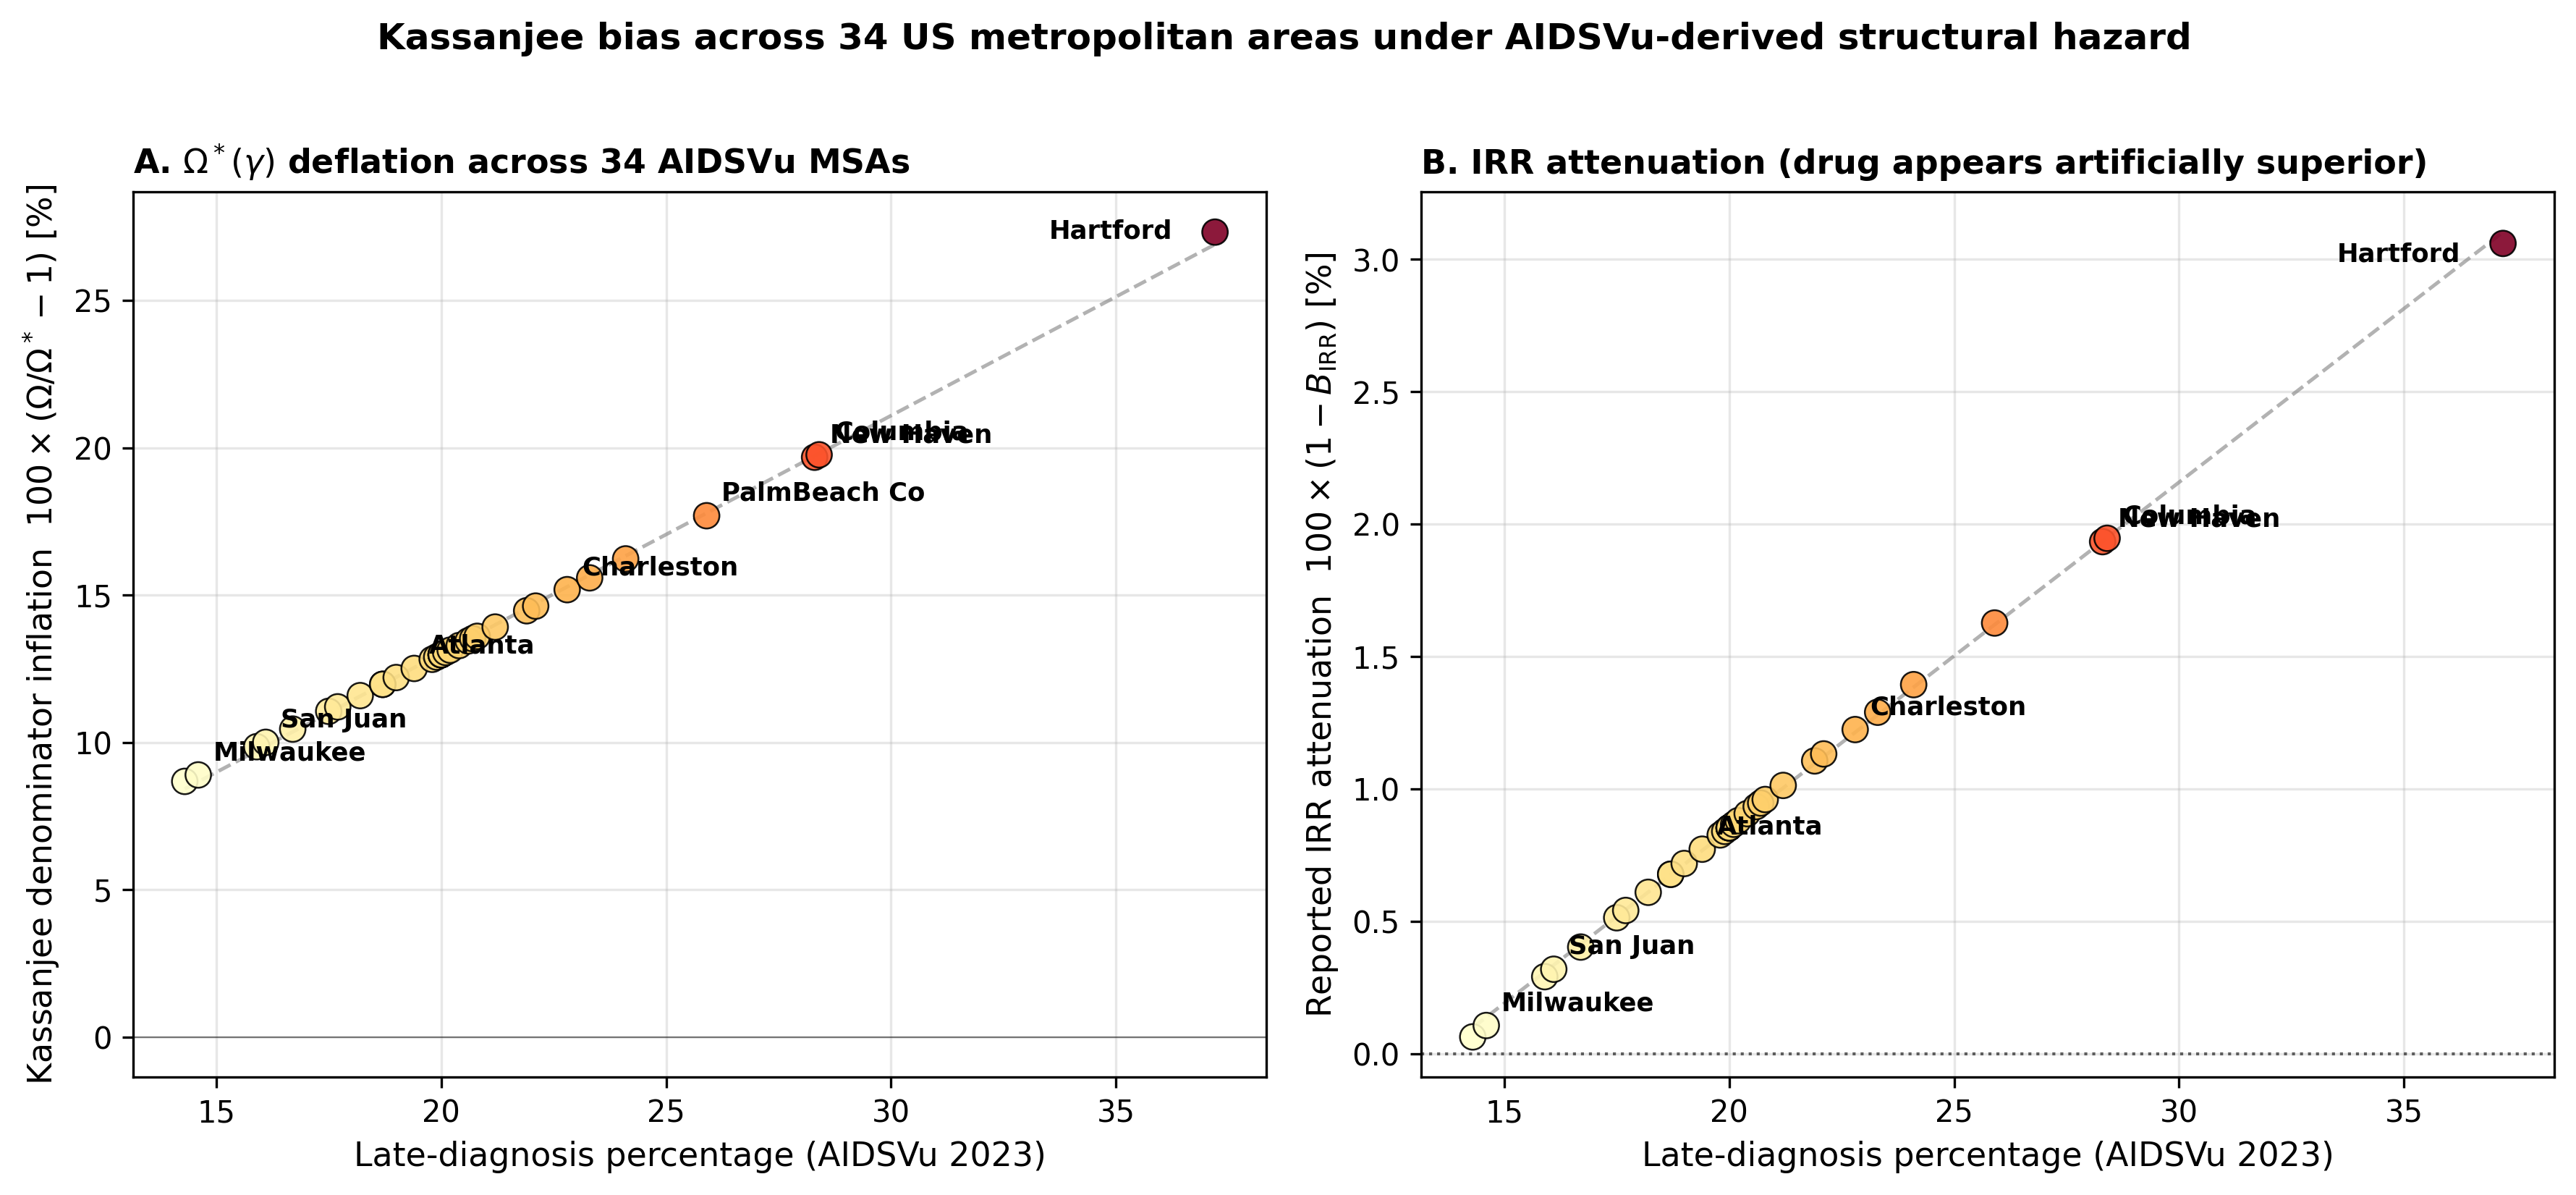
\includegraphics[width=0.95\textwidth]{Figure1_KassanjeeBias.png}
\caption{Kassanjee bias across 34 US high-burden metropolitan areas under AIDSVu-derived structural hazard. \textbf{Panel~A:} $\Omega^*(\gamma)$ deflation as a function of AIDSVu late-diagnosis percentage. Denominator inflation ranges from 8.7\% (Milwaukee) to 27.3\% (Hartford). \textbf{Panel~B:} Joint reported-IRR attenuation $100 \times (1 - B_{\mathrm{IRR}})$, reflecting the net bias after accounting for intervention-arm retention loss and cross-sectional screening-cohort censoring. Both panels display monotone scaling with late-diagnosis severity, demonstrating the structural nature of the bias rather than stochastic variation.}
\label{fig:main}
\end{figure}

\subsection{What the distribution shows}

Three features of the distribution are worth naming explicitly.

First, the bias is not negligible in the high-severity tail. A 27\% denominator inflation is substantially larger than the calibration uncertainty typically acknowledged for the Sedia LAg-EIA in Gao-framework sensitivity analyses.

Second, the bias is structured---monotone in late-diagnosis percentage, which is itself monotone in the structural-testing-avoidance substrate. Cities with the worst late-diagnosis indicators are cities with the largest correction. Any claim of efficacy transportability across these cities must account for heterogeneous bias in the estimator, not merely heterogeneous biology of the populations.

Third, the correction applies even at the low-severity end. Even Milwaukee, the best-performing city in the dataset, shows an 8.7\% denominator inflation. The closed-system assumption fails at every city; the magnitude simply scales with structural context.

\subsection{Transportability implications}

A trial reporting IRR = 0.04 (96\% efficacy) in an aggregate analysis across cohorts with $\gamma_{\mathrm{enrolled}}$ concentrated at the low-severity end of the distribution cannot have that IRR applied without correction to deployment populations at the high-severity end. The Kassanjee bias factor differs by approximately 3 percentage points across the full AIDSVu range---small relative to the primary biological constraints on transportability~\cite{demidont2026fw} but non-trivial for populations at the margin of clinical and regulatory decisions.

\section{Implications and prospective correction}

\subsection{For completed trials}

Published IRR estimates should be read as conditional on the enrolled cohort's structural hazard profile, with the understanding that transportability to deployment populations requires explicit consideration of whether the deployment population's hazard profile differs from the enrolled cohort's. For populations at the high-severity end of the AIDSVu distribution, the correction factor is non-negligible and should be reported alongside the uncorrected estimate.

\subsection{For prospective trial design}

Three recommendations follow for cross-sectional incidence cohorts in future prevention trials:

(i) The Statistical Analysis Plan should specify the structural hazard profile of the enrolled Incidence Phase cohort using population-level surveillance indicators available at screening---minimally, late-diagnosis percentage for the catchment population.

(ii) The primary analysis should report both the standard Kassanjee/Gao estimate and a $\Omega^*(\gamma)$-corrected estimate, with $\gamma$ estimated from the catchment population's surveillance profile. The correction does not require modifying the estimator itself; it is a post-hoc adjustment to the nominal MDRI. Variance propagation follows from the Gao 2021 delta-method formulation with an additional variance component $\sigma^2_\gamma$.

(iii) Where eligibility criteria include a testing-interval exclusion, the SAP should explicitly acknowledge the selection mechanism and report the cohort's enrolled hazard under an assumed or empirically estimated amplification factor relative to the catchment population.

\subsection{For regulatory interpretation}

Regulatory agencies evaluating efficacy claims from counterfactual-controlled prevention trials should consider requesting, as part of standard review, explicit documentation of the enrolled cohort's structural hazard profile and its relationship to the deployment population envisioned in the proposed label. Where these profiles differ substantially, the efficacy claim should be annotated with the appropriate Kassanjee correction factor.

\subsection{Limitations}

Four limitations warrant acknowledgment. First, the closed-form correction relies on an exponential approximation of $P_R(t)$; exact correction under the published LAg-EIA calibration would produce somewhat larger $\Omega^*$ deflations. The closed-form is conservative. Second, the parameterization of $\gamma_{\mathrm{city}}$ from late-diagnosis percentage is a one-variable approximation; richer parameterizations are straightforward extensions. Third, the assumption that $\gamma$ acts identically on recently-infected and uninfected individuals within the screening window is a first-order approximation. Fourth, the 1.5$\times$ selection amplification factor is derived from plausible bimodal testing-behavior models rather than direct empirical measurement; direct estimation using participant-level testing-interval data from completed trials would refine this factor.

None of these limitations reverses the directional claim. The correction is conservative in all four dimensions.

\subsection{Conclusion}

The Kassanjee cross-sectional incidence estimator is a powerful and broadly adopted tool in contemporary prevention-trial epidemiology. Its validity depends on a closed-system assumption that is systematically violated in populations experiencing structural censoring, and the violation is compounded by trial-design selection mechanisms that recruit the Incidence Phase cohort specifically on the testing-engagement axis that drives the underlying hazard. The bias is quantifiable, corrigible, and can be addressed prospectively in trial design without modifying the estimator itself.

The correction matters most for the populations who can least afford to have their prevention needs misestimated---those whose structural context produces both elevated risk and elevated measurement bias. Responsible use of RITA-based incidence estimation in these populations requires explicit acknowledgment of the calibration-to-deployment mismatch and transparent reporting of corrected estimates alongside the conventional ones. The conventional practice---applying a validation-cohort $\Omega$ without correction---is no longer defensible for populations with substantially elevated structural hazard relative to the calibration set.

\section*{Author contributions}
A.C.D.: conceptualization, formal analysis, mathematical derivation, numerical computation, figure generation, manuscript drafting. Sole author.

\section*{Acknowledgments}
The author thanks the HIV prevention research community whose published work informed parameter calibration.

\section*{Funding}
No external funding was received. Work conducted under the affiliation of Nyx Dynamics LLC, of which the author is sole owner.

\section*{Competing interests}
The author reports prior employment with Gilead Sciences, Inc., from January 2020 through November 2024; all Gilead stock was fully divested by December 2024. Employment ended prior to initiation of this research. Gilead Sciences had no role in conception, analysis, interpretation, writing, or the decision to submit.

\section*{Data and code availability}
All code and data-processing scripts are available at \url{https://github.com/Nyx-Dynamics/Kassanjee-Structural-Bias} (Zenodo DOI: \href{https://doi.org/10.5281/zenodo.19733583}{10.5281/zenodo.19733583}). The AIDSVu 2023 dataset is publicly available at \url{https://aidsvu.org}. No individual-level data were used.

\section*{AI tool disclosure}
Computational analyses were conducted in Python (NumPy, SciPy, Matplotlib, pandas). Large language models (Anthropic Claude) were used to support manuscript drafting and readability. All AI tools were used as assistive technologies only. The author retains full responsibility for design, analysis, interpretation, and conclusions.

\begin{thebibliography}{99}
\small
\bibitem{kassanjee2012} Kassanjee R, McWalter TA, Barnighausen T, Welte A. A new general biomarker-based incidence estimator. \emph{Epidemiology}. 2012;23(5):721--728.

\bibitem{gao2021} Gao F, Glidden DV, Hughes JP, Donnell DJ. Sample size calculation for active-arm trial with counterfactual incidence based on recency assay. \emph{Statistical Communications in Infectious Diseases}. 2021;13(1):20200009.

\bibitem{bekker2024} Bekker L-G, Das M, Abdool Karim Q, et al. Twice-yearly lenacapavir or daily F/TAF for HIV prevention in cisgender women. \emph{N Engl J Med}. 2024;391(13):1179--1192.

\bibitem{kelley2025} Kelley CF, Acevedo-Quinones M, Agwu AL, et al. Twice-yearly lenacapavir for HIV prevention in men and gender-diverse persons. \emph{N Engl J Med}. 2025;392(14):1261--1276.

\bibitem{aidsvu2023} AIDSVu. Downloadable datasets for US metropolitan statistical areas. Rollins School of Public Health, Emory University. 2023. Accessed at \url{https://aidsvu.org}.

\bibitem{sedialag} Sedia Biosciences Corporation. HIV-1 LAg-Avidity EIA: Assay package insert and calibration documentation. Portland, OR. Current revision.

\bibitem{cdcatp2023} Centers for Disease Control and Prevention. Monitoring Selected National HIV Prevention and Care Objectives by Using HIV Surveillance Data---United States and 6 Dependent Areas, 2023. \emph{HIV Surveillance Supplemental Report}. 2023.

\bibitem{nhbs2023} Centers for Disease Control and Prevention. HIV infection, risk, prevention, and testing behaviors among persons who inject drugs---National HIV Behavioral Surveillance. 2023.

\bibitem{bjs2023} Bureau of Justice Statistics. Prisoners in 2022---Statistical Tables. US Department of Justice. 2023.

\bibitem{demidont2026fw} Demidont AC. Finite prevention windows for HIV post-exposure prophylaxis: Irreversible proviral integration defines route-specific intervention limits. \emph{Under review}. 2026.
\end{thebibliography}

\end{document}
